% Appendix
\chapter{Appendix}


\seb{change appendix name or way it is displayed. I want to have just 1 appendix}
%===============================================================================
\section{Additional material}\label{sec:additional_material}
%===============================================================================
\noindent The \citetalias{octave_community_gnu_2018} fswof2d package can be downloaded at:
\begin{itemize}
\itemsep0em
  \item \url{https://bitbucket.org/binello7/fswof2d/}
\end{itemize}

\noindent All of the material composing these thesis (documents, scripts, files, functions, etc.) is available at:
\begin{itemize}
\itemsep0em
  \item \url{https://bitbucket.org/binello7/master_thesis}
\end{itemize}



%===============================================================================
\section{Case study 1}
%===============================================================================
\begin{figure}[H]
  \centering
  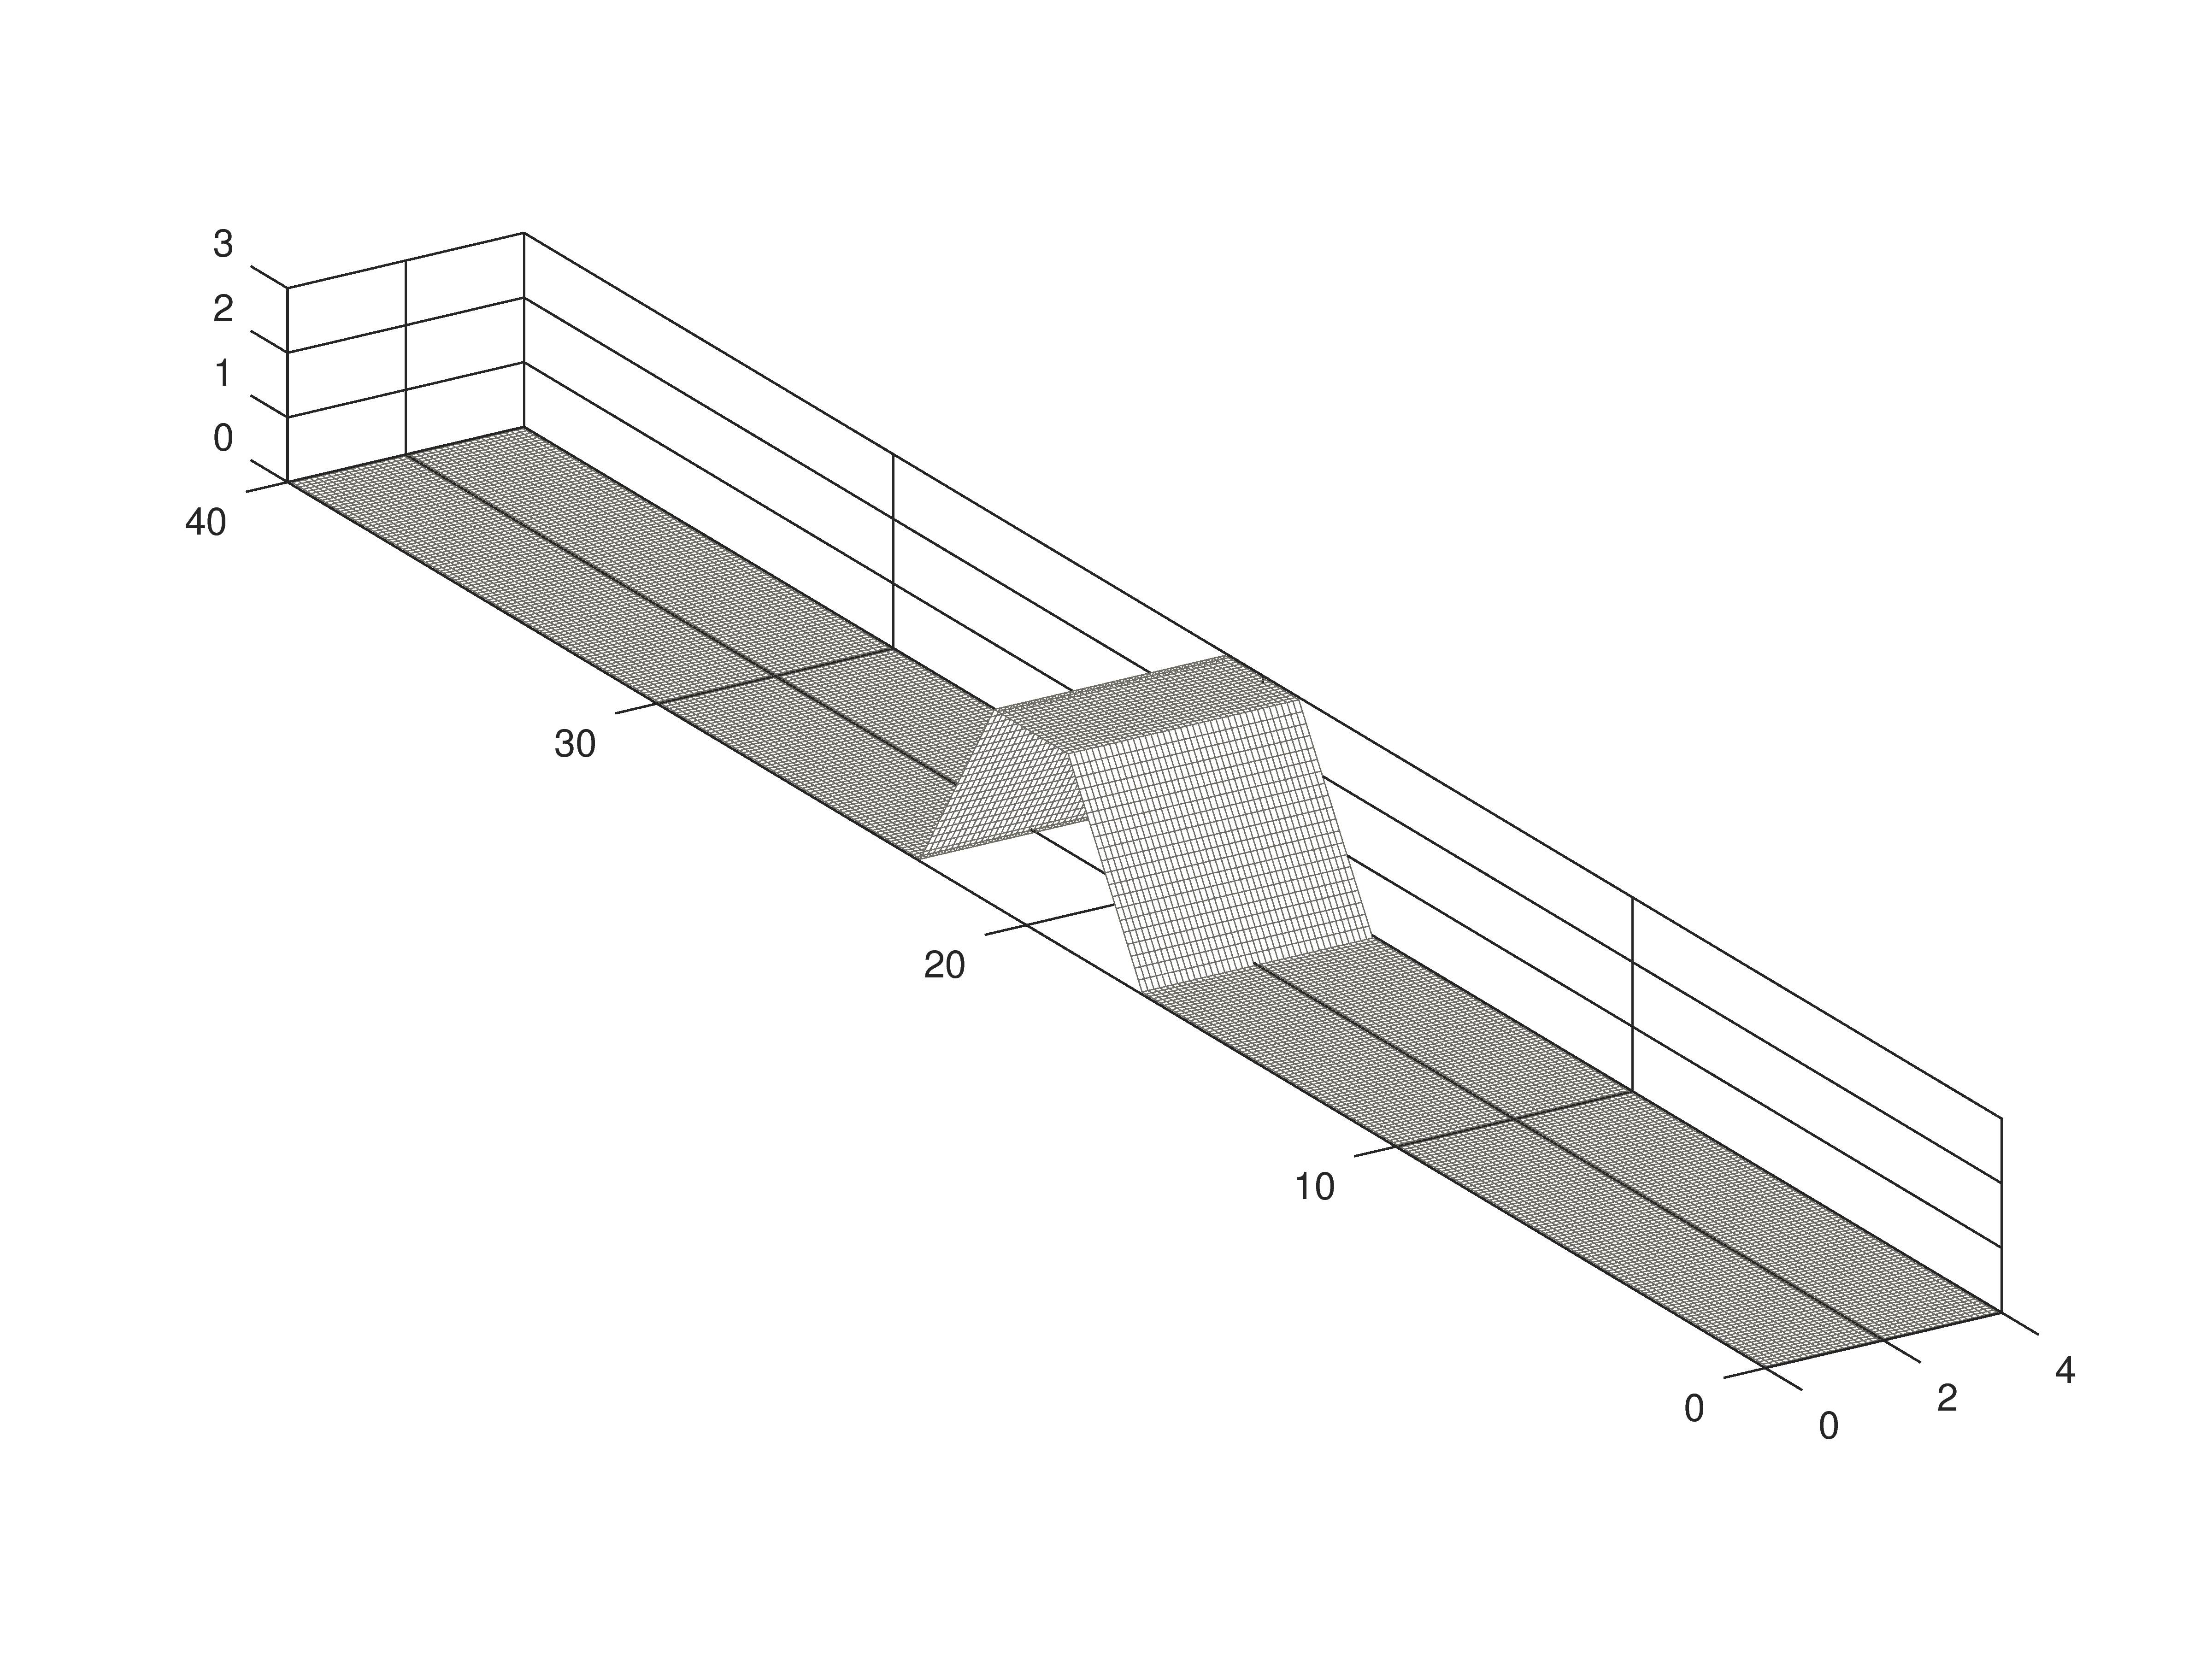
\includegraphics[width=0.8\textwidth]{Figures/channel.png}
  \caption{Topography of the channel used for \emph{case study 1}. The channel presents no walls because "wall boundary conditions" were chosen in \textit{FullSWOF\_2D} for the two lateral boundaries.}
  \label{fig:channel}
\end{figure}
\seb{does it make sense to put this figure?}
\seb{change the caption of the figure!}


\begin{figure}[H]
  \centering
  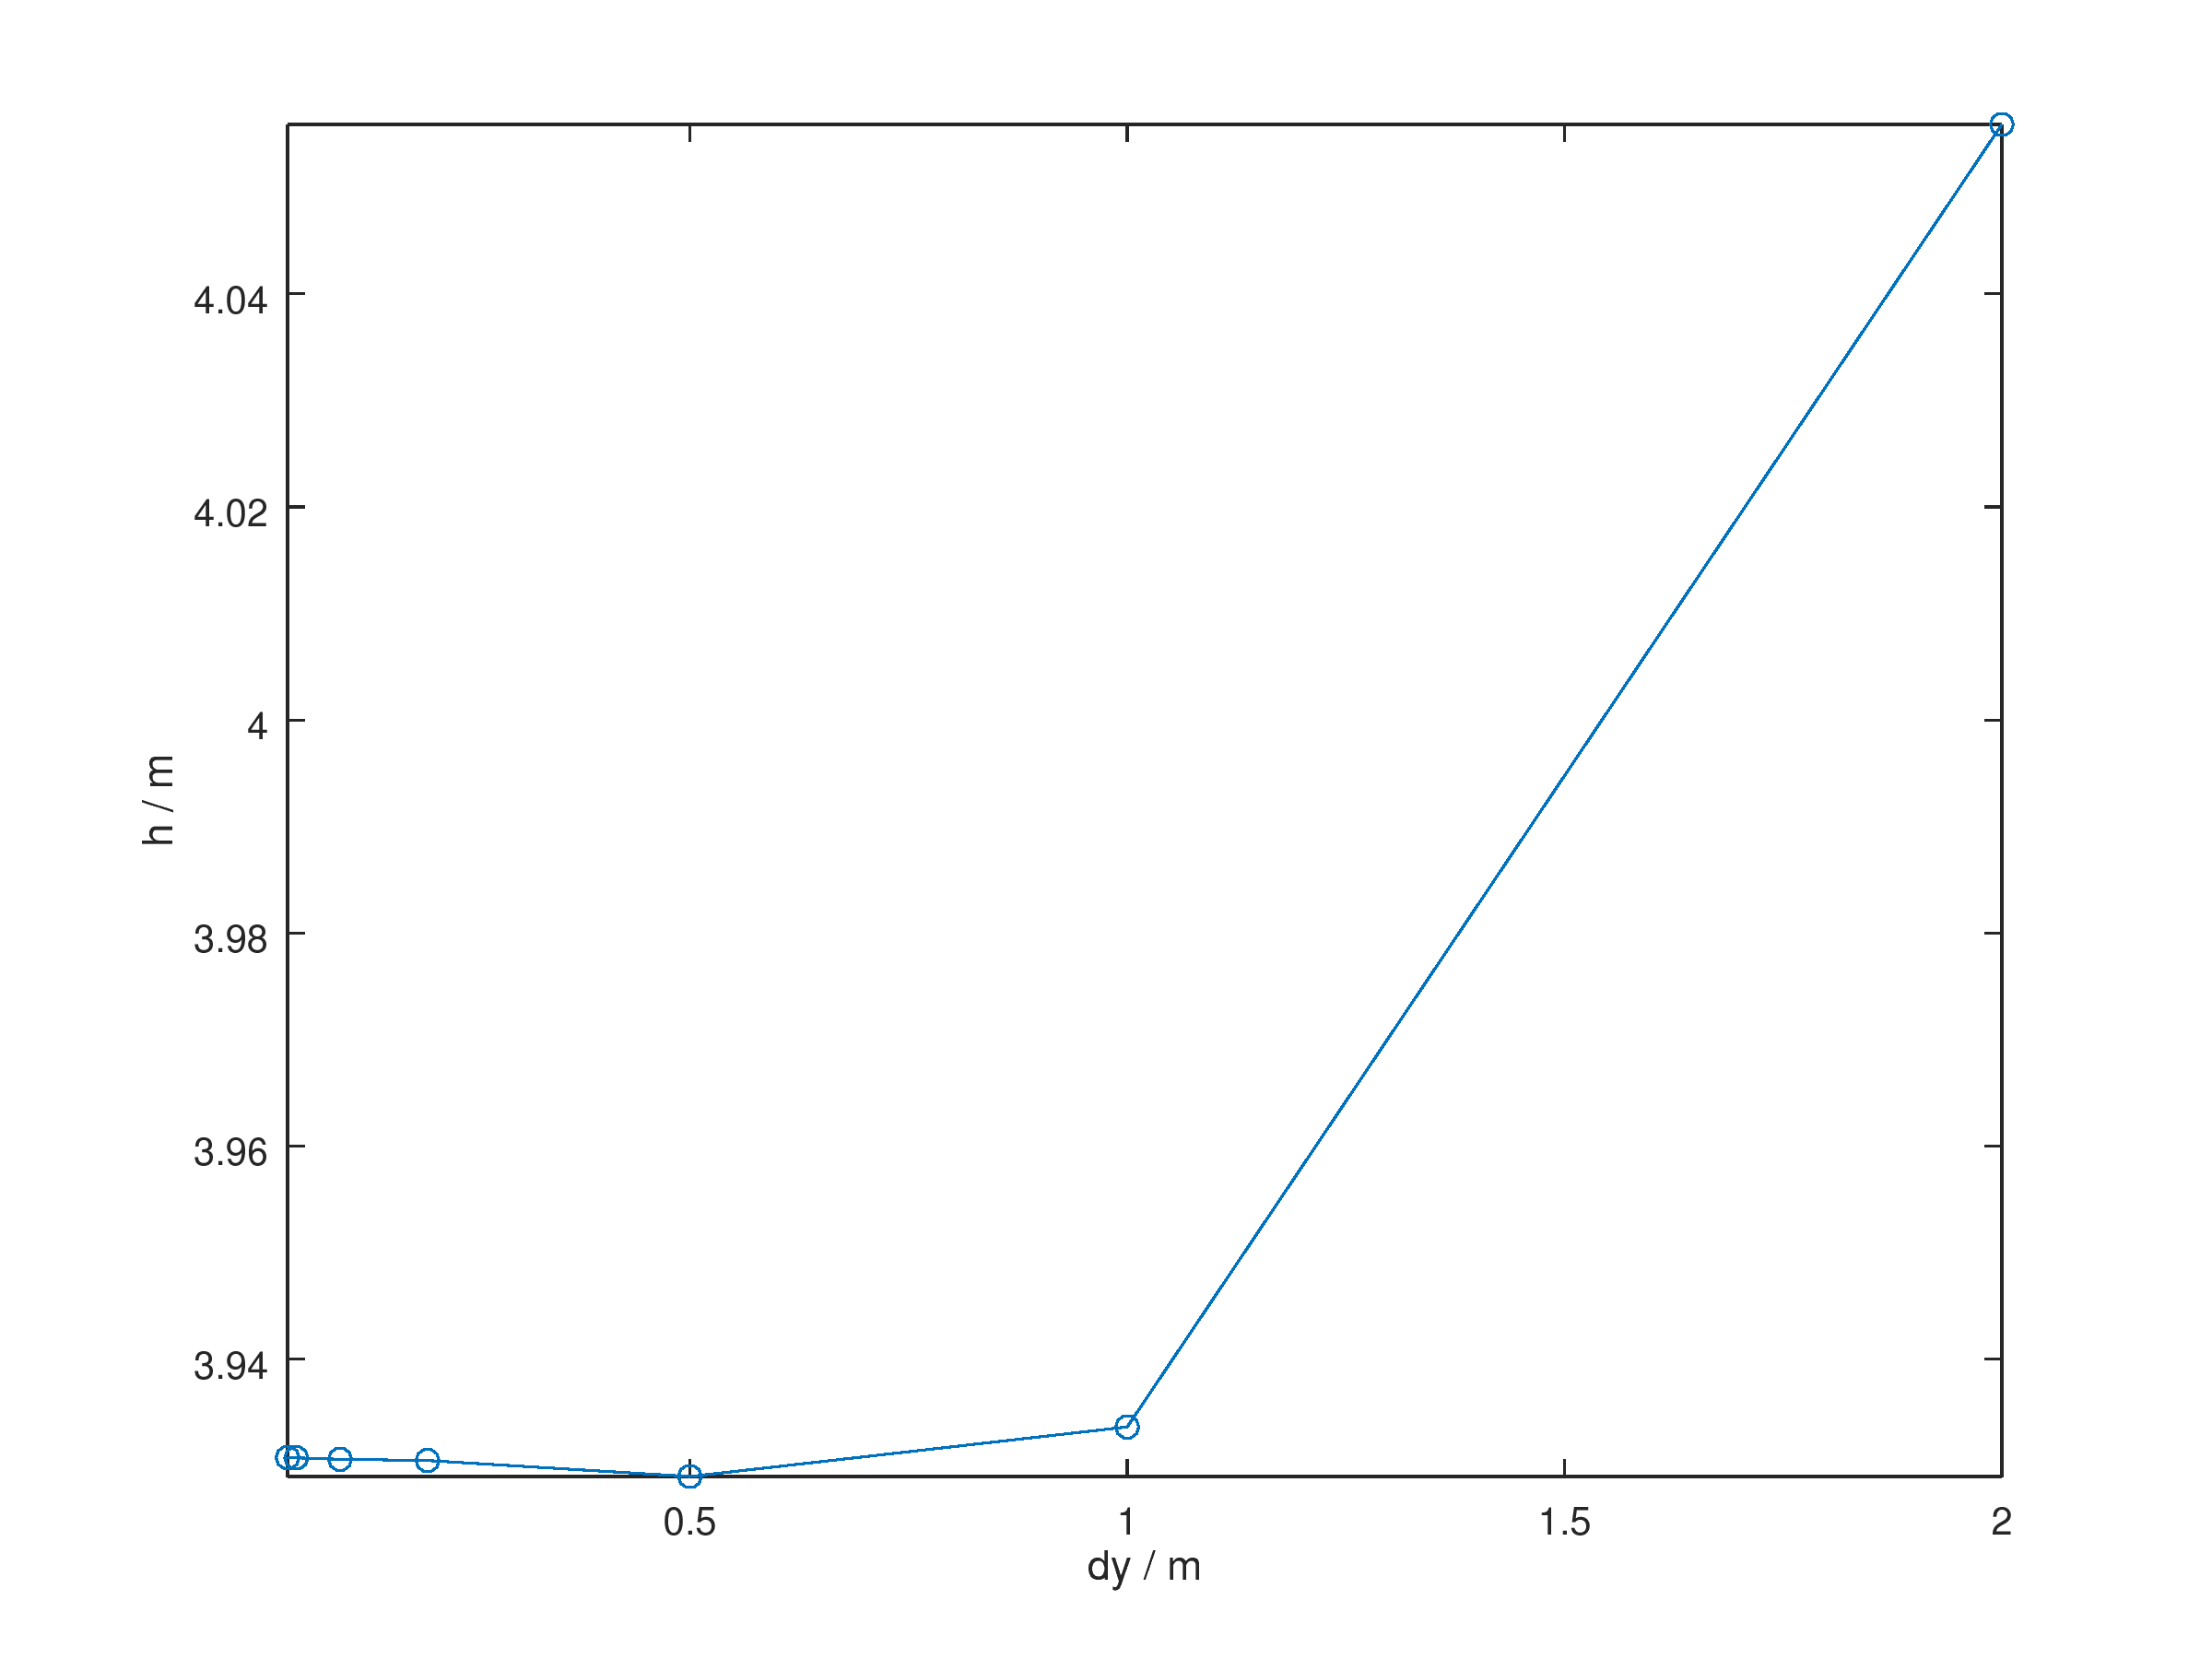
\includegraphics[width=0.7\textwidth]{Figures/convergence_center.png}
  \caption{Measured free surface height at the weir crest as a function of the grid resolution used.}
  \label{fig:convergence_center}
\end{figure}


\begin{table}[H]
  \centering
  \caption{Dataset used for computing the model error.}
  \label{tab:dataset_error}
  \begin{adjustbox}{max width=\textwidth}
    \begin{tabular}{lrrrrrrrrrrrrrr}
      \toprule
      $\bm{h_w}\,/\si{\m}$             & 0.00 & 0.50 & 0.55 & 0.61 & 0.66 & 0.80 & 0.89 & 0.93 & 1.05 & 1.08 & 1.20 & 1.16 & 1.27 & 1.30\\
      $\bm{Q}$\,/\si{\cubic\m\per\s}   & 0.00 & 2.16 & 2.58 & 2.99 & 3.40 & 4.64 & 5.46 & 5.88 & 7.11 & 7.53 & 8.76 & 8.35 & 9.59 & 10.00\\
      \bottomrule
    \end{tabular}}
  \end{adjustbox}
\end{table}


\begin{figure}[H]
  \centering
  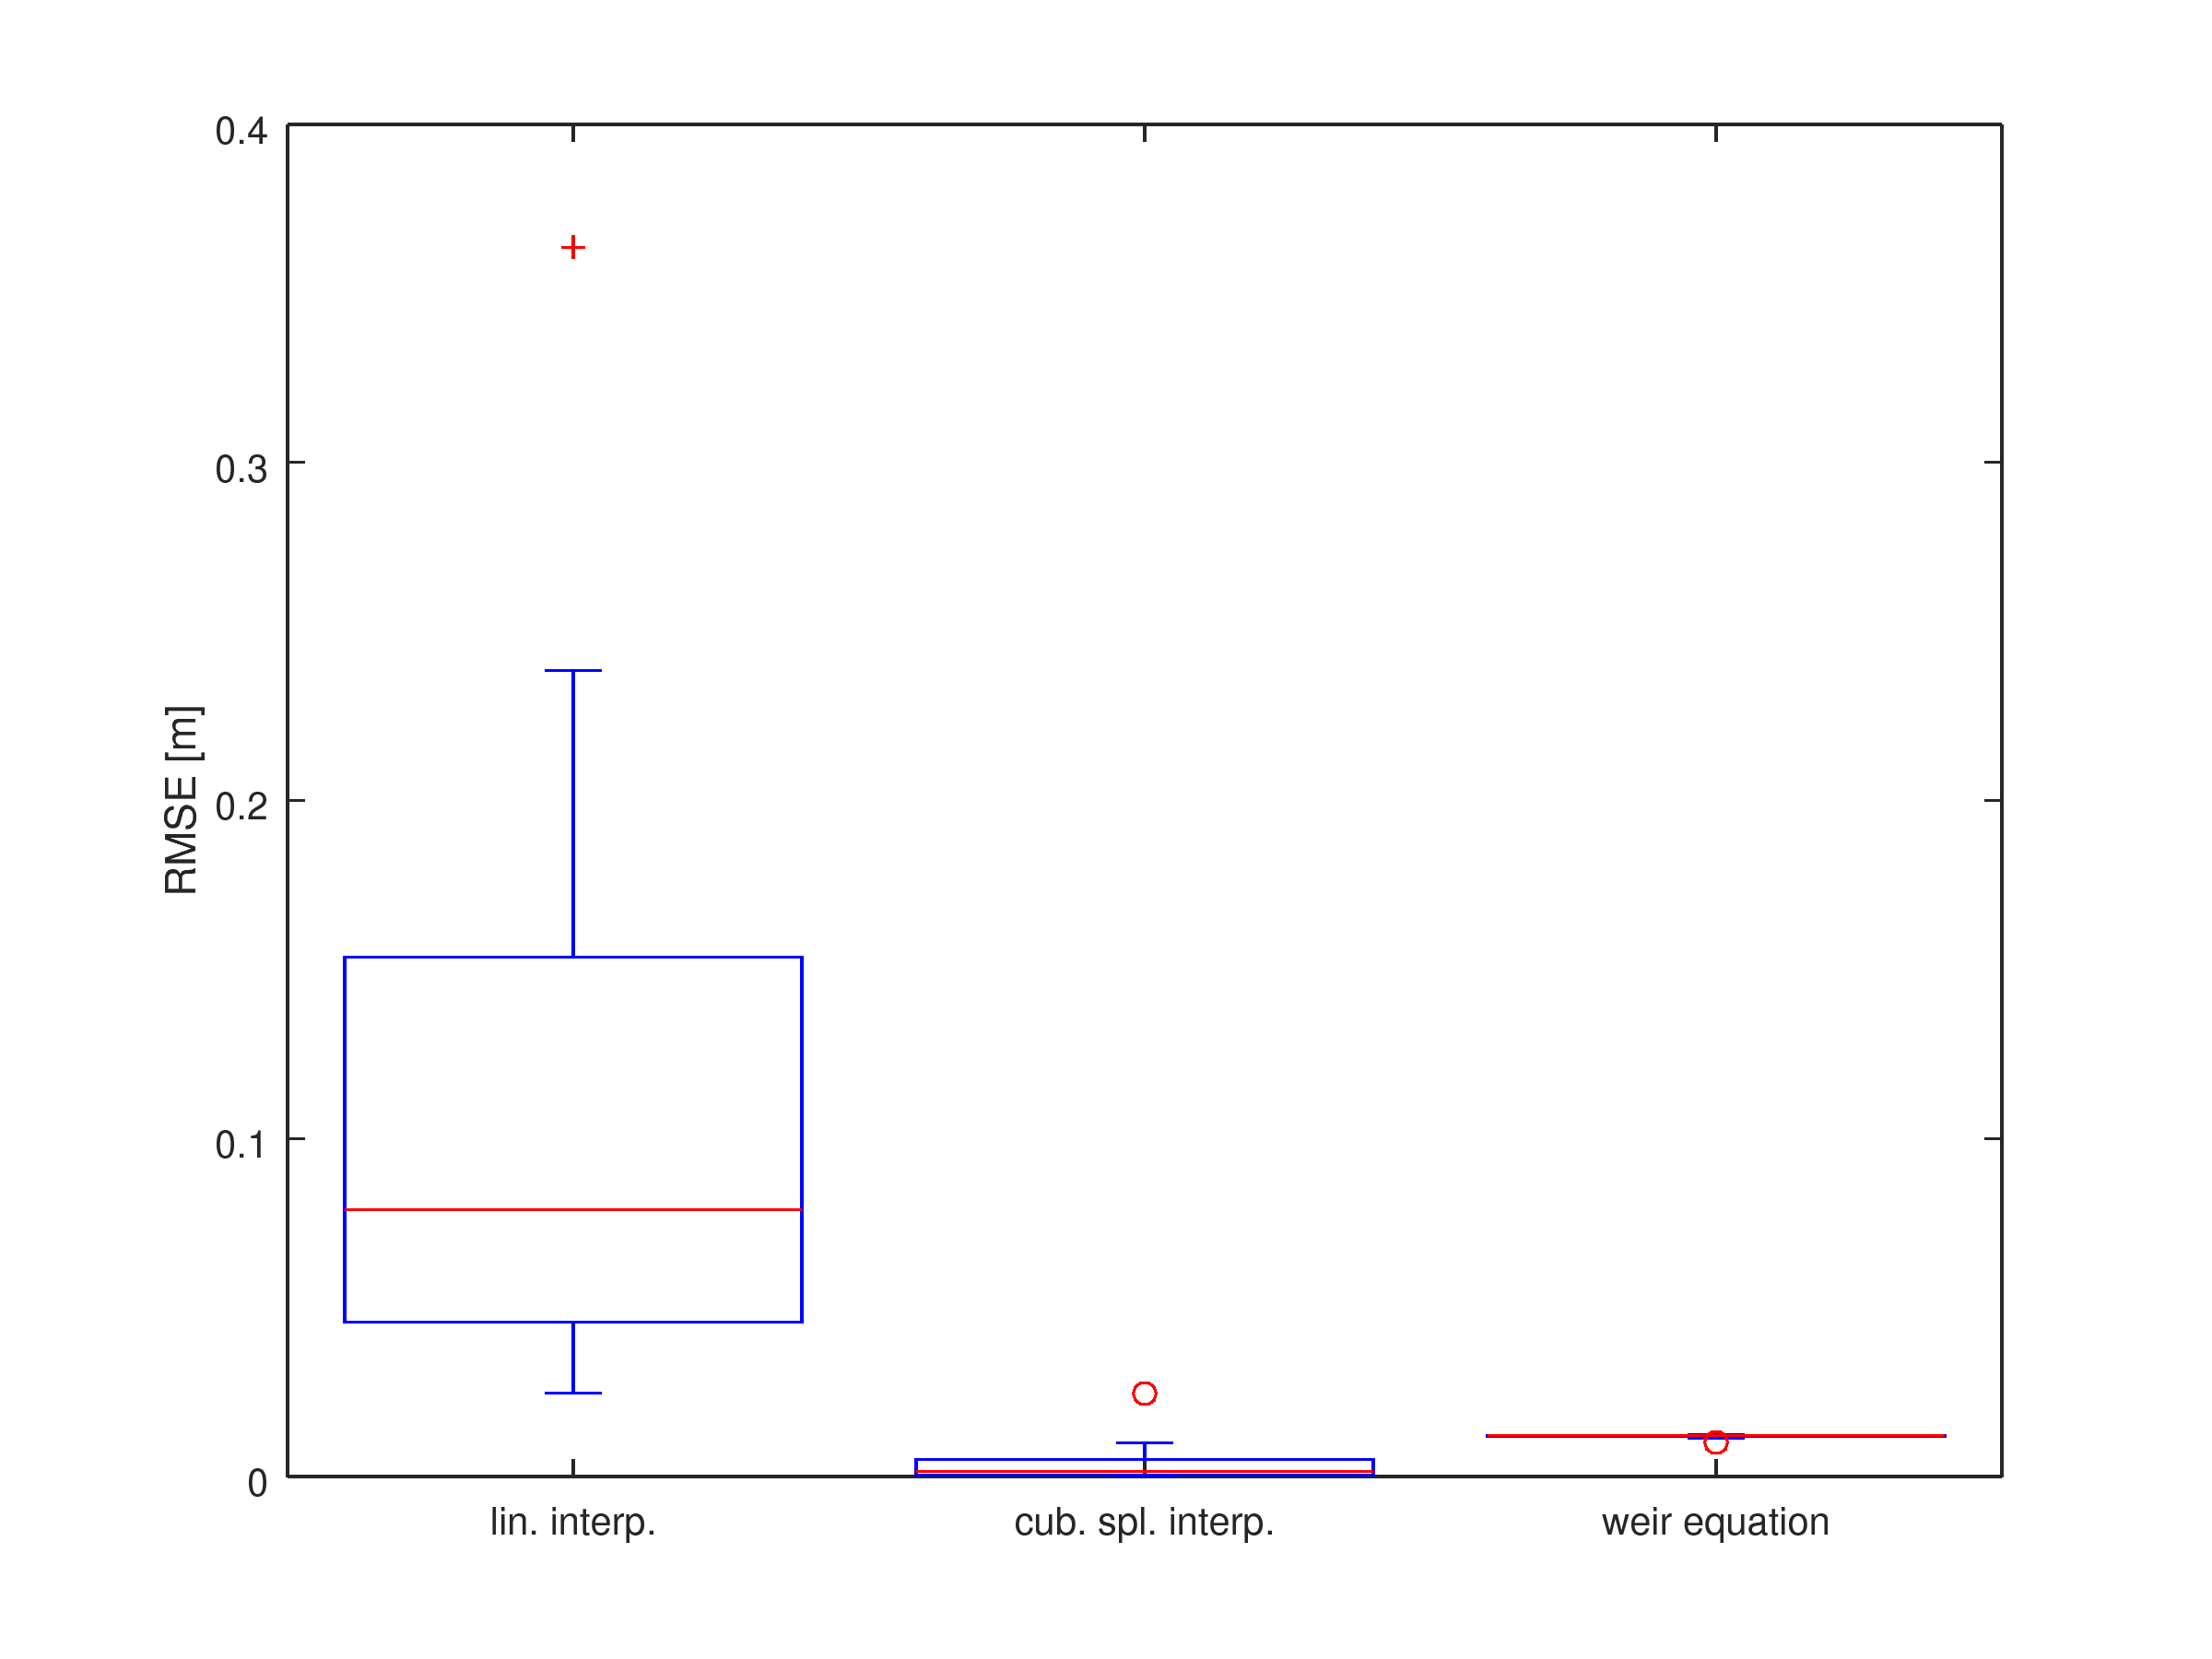
\includegraphics[width=0.7\textwidth]{Figures/boxplot_models.png}
  \caption{Box plot summarizing the performance of the three models by using $[\numrange{4}{13}]$ \# of points. The red line represent the median RMSE. The box is given by the \nth{1} and \nth{3} quartile. Whiskers are drawn at $1.5 \times IQR$. Points between $1.5 \times IQR$ and $3 \times IQR$ are marked with 'o', while '+' indicates points beyond this range \autocite{eaton_gnu_2016}.}
  \label{fig:boxplot_models}
\end{figure}

%===============================================================================
\section{Case study 2}
%===============================================================================
%-------------------------------------------------------------------------------
\subsection{Test dataset}\label{sec:test_dataset}
%-------------------------------------------------------------------------------
\inputminted[
  fontsize=\footnotesize,
  firstline=50,
  lastline=67,
  numbersep=2pt,
  gobble=0,
  frame=none,
  bgcolor=light-gray,
  framesep=10mm
]{octave}{code.m}

%-------------------------------------------------------------------------------
\subsection{Validation dataset}
%-------------------------------------------------------------------------------
\begin{table}[H]
  \centering
  \caption{Dataset used for the validation of the emulator.}
  \label{tab:validation_dataset}
  \begin{tabular}{ccccccc}
    \toprule
     & \textbf{1} & \textbf{2} & \textbf{3} & \textbf{4} & \textbf{5} & \textbf{6} \\
    \midrule
    $\bm{I}$ {\scriptsize[\si{\milli\meter\per\hour}]} & 15  & 20  & 22  & 25  & 25  & 35\\
    $\bm{\theta_i}$                                    & 0.9 & 0.2 & 0.5 & 0.8 & 0.4 & 0.8\\
    \bottomrule
  \end{tabular}
\end{table}

%-------------------------------------------------------------------------------
\subsection{Classification additional dataset}
%-------------------------------------------------------------------------------
\begin{table}[H]
  \centering
  \caption{Dataset used for the second, more accurate classification.}
  \label{tab:classification_dataset}
  \begin{tabular}{ccccccccc}
    \toprule
    $\bm{I}$ {\scriptsize[\si{\milli\meter\per\hour}]} & 11.2  & 12.0  & 13.5  & 14.7  & 15.4  & 15.8 & 16.3 & 17.0\\
    $\bm{\theta_i}$                                    & 0.95  & 0.80  & 0.60  & 0.45  & 0.35  & 0.3  & 0.20 & 0.05\\
    \bottomrule
  \end{tabular}
\end{table}


\begin{figure}[H]
  \centering
  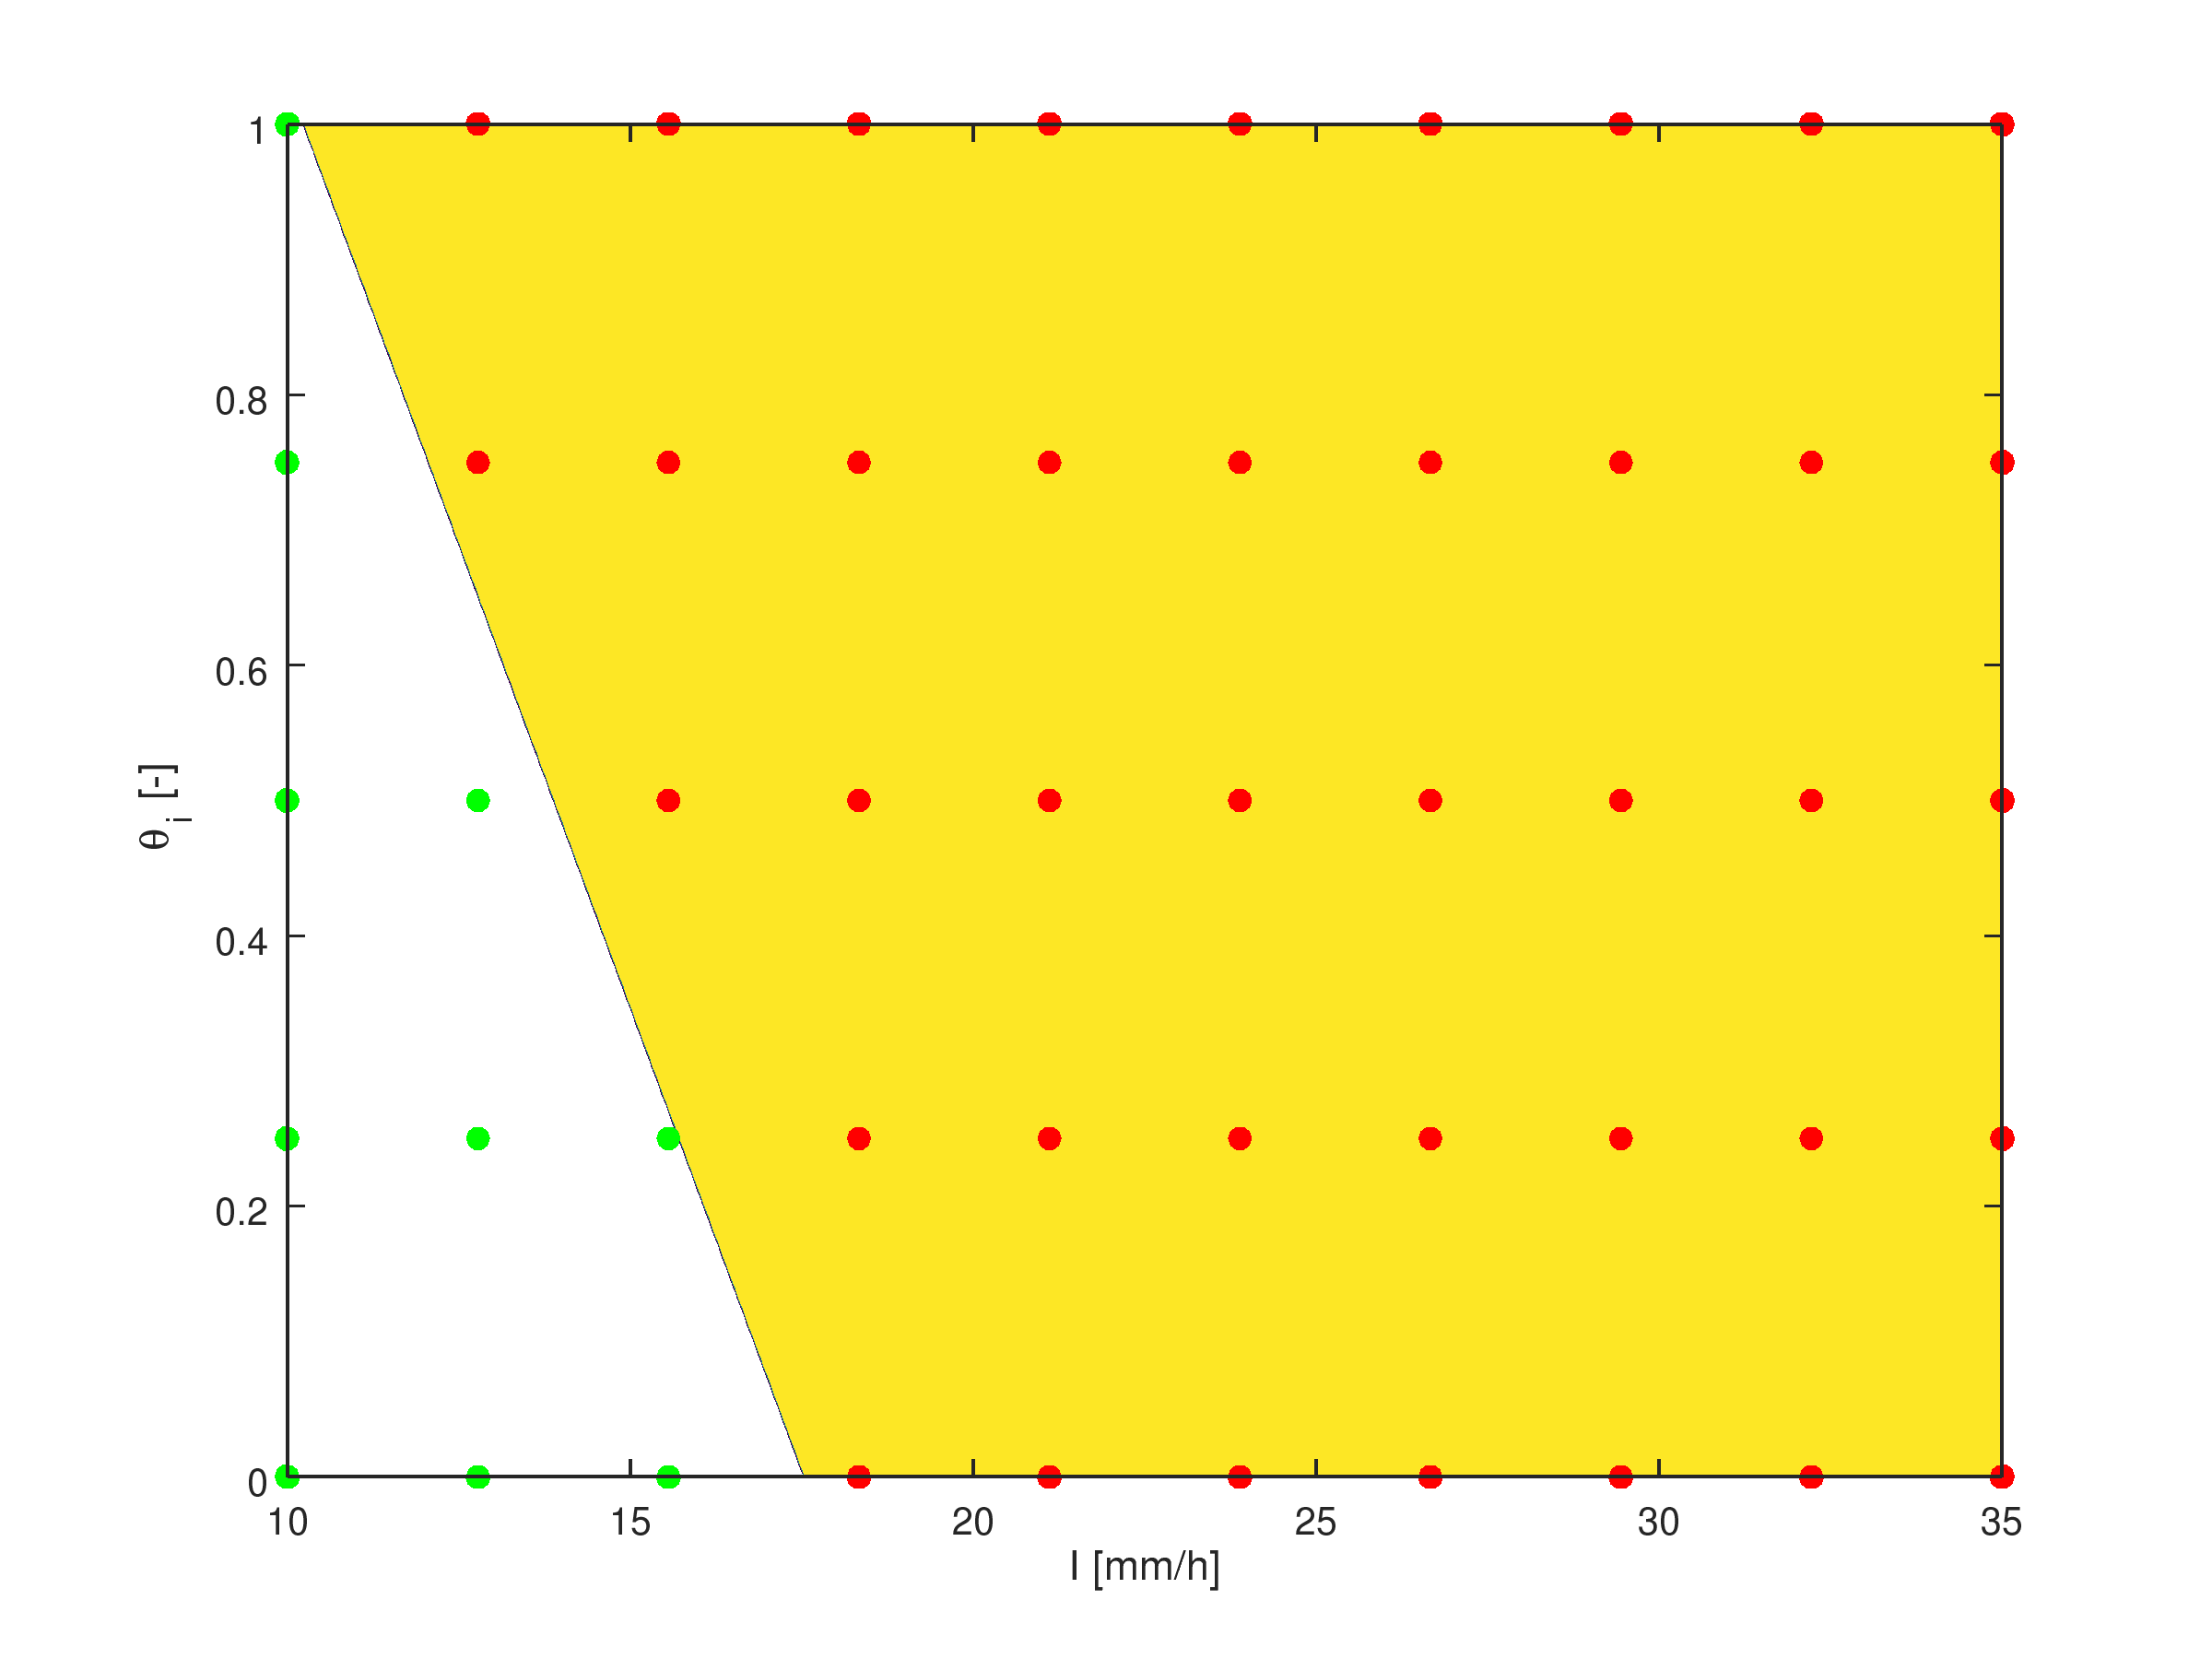
\includegraphics[width=0.7\textwidth]{Figures/classifier_trn.png}
  \caption{Linear separation of the training dataset with use of the "meanLinear" and "covConst" functions of the \citetalias{rasmussen_gaussian_2010} package.}
  \label{fig:classifier_trn}
\end{figure}

%-------------------------------------------------------------------------------
\subsection{Values of classifier's hyperparameters}\label{sec:classifier_hyperparameters}
%-------------------------------------------------------------------------------
\inputminted[
  fontsize=\footnotesize,
  firstline=115,
  lastline=132,
  numbersep=2pt,
  gobble=0,
  frame=none,
  bgcolor=light-gray,
  framesep=10mm
]{octave}{code.m}


%-------------------------------------------------------------------------------
\subsection{Values of emulator's hyperparameters}\label{sec:emulator_hyperparameters}
%-------------------------------------------------------------------------------
\inputminted[
  fontsize=\footnotesize,
  firstline=91,
  lastline=108,
  numbersep=2pt,
  gobble=0,
  frame=none,
  bgcolor=light-gray,
  framesep=10mm
]{octave}{code.m}


%-------------------------------------------------------------------------------
\subsection{Detailed validation performance}
%-------------------------------------------------------------------------------
\begin{table}[H]
  \centering
  \caption{Emulator performance on every validation point.}
  \label{tab:validation_performance}
  \begin{tabular}{lcccccc}
    \toprule
     & \textbf{1} & \textbf{2} & \textbf{3} & \textbf{4} & \textbf{5} & \textbf{6}\\
    \midrule
    \textbf{simulated} $\bm{t_!}\,[\si{\minute}]$     & 91.5 & 192.5 & 101.5 & 32.5 & 32.5 & 11.5\\
    \textbf{emulated}  $\bm{t_!}\,[\si{\minute}]$     & 86.2 & 198.0 & 95.5  & 32.4 & 34.0 & 11.0\\
    \textbf{error}     $\bm{\epsilon}\,[\si{\minute}]$ & 5.3  & -5.5  & 6.0   & 0.1  & -1.5 & 0.5\\
    \bottomrule
  \end{tabular}
\end{table}
